\documentclass[12pt]{article}

% ── layout ───────────────────────────────────────────────────────────────────
\usepackage[margin=1in]{geometry}
\usepackage{setspace}
\onehalfspacing

% ── font (newpx on Overleaf; Palatino fallback elsewhere) ────────────────────
\IfFileExists{newpxtext.sty}{\usepackage{newpxtext,newpxmath}}{\usepackage{mathpazo}}

% ── packages ─────────────────────────────────────────────────────────────────
\usepackage{amsmath,amssymb}
\usepackage{booktabs}
\usepackage{threeparttable}
\usepackage{graphicx}
\usepackage{float}
\usepackage{microtype}
\usepackage[dvipsnames]{xcolor}
\usepackage{natbib}
\usepackage[colorlinks=true,linkcolor=BurntOrange,citecolor=BurntOrange,urlcolor=BurntOrange]{hyperref}

\setlength{\parskip}{0.4em}

% ─────────────────────────────────────────────────────────────────────────────
\title{\textbf{Rankings, Attention, and Bookings}\\[4pt]
       \large Evidence from Expedia's Random Ordering Experiment}
\author{Dili Maduabum\thanks{University of Michigan. Code and replication files: \url{https://github.com/dmaduabum/expedia-causal}.}}
\date{April 2026}
% ─────────────────────────────────────────────────────────────────────────────

\begin{document}
\maketitle

\begin{abstract}
\noindent
Online platforms decide which products consumers see first, but the effect of a product's position on what consumers consider and buy is difficult to measure, because platforms place the products they expect consumers to prefer at the top. I study this question in a setting where the link between position and product is broken: searches in which Expedia displayed hotels in random order. Comparing hotels on the same randomly ordered page, I find that moving a hotel from the first to the fifth position reduces its click and booking rates by about half, and moving it from first to tenth reduces them by about two-thirds. Among hotels that are clicked, booking rates vary little with position, a pattern consistent with position affecting purchases mainly through which products consumers consider. Position effects are largest for hotels priced below others on the same page.
\end{abstract}

\clearpage

% =============================================================================
\section{Introduction}
% =============================================================================

Every time a traveler searches for a hotel on Expedia, a ranking algorithm determines which properties appear first. Because attention is highly concentrated at the top of the results page, this ranking can strongly shape which hotels are clicked and booked. But the hotels shown first are also the ones the algorithm expects consumers to like, so the advantage of appearing at the top is difficult to separate from the advantage of being a better hotel.

Expedia created variation that separates the two. For about 30 percent of searches, the platform displayed hotels in random order instead of using its ranking algorithm. On random pages listing at least 25 hotels, the first listing is clicked about 12 percent of the time, the fifth about 5 percent, the tenth about 4 percent, and the twenty-fifth about 2 percent. Because a hotel's position was assigned by chance, this decline reflects how consumers move down a page, not which hotels were placed first.

I use these searches to answer three questions. How much does a hotel lose by appearing lower on the page? Does position mainly affect which hotels consumers consider, or also what they choose once they have considered a hotel? And which hotels depend most on favorable placement?

Because the data record both clicks and bookings, they provide some evidence on where in the purchase process position matters. If position mainly determines which hotels consumers notice, moving a hotel down the page should reduce its clicks and, as a consequence, its bookings, but among hotels that consumers click, booking rates need not vary with position. If consumers also read position as information about quality, a hotel shown lower on the page should be less likely to be booked even after it is clicked.

The position effects are large and concentrated near the top of the page. Moving a hotel from first to fifth position reduces its click rate by 53 percent and its booking rate by 51 percent. Moving it from fifth to tenth reduces the two rates by a further 32 and 37 percent. Overall, a hotel moved from first to tenth position loses about two-thirds of its clicks and bookings.

The evidence also points to attention as the main channel. Among hotels that consumers click, booking rates vary little with position: ten positions lower is associated with a change in booking probability of $-0.04$ percentage points, with a standard error of 0.22. This comparison is not causal, because clicking is itself affected by position, but the pattern is consistent with most of the booking effect operating through which hotels consumers consider.

Finally, position matters more for some hotels than for others. Hotels priced below the median of their search lose 51 percent of their mean click rate per ten positions, compared with 42 percent for hotels priced above it. Relative position effects are much more similar for chain and independent hotels, and across star ratings and review scores.

This paper relates to work measuring position effects in online markets, including \citet{ghose2014examining} and \citet{narayanan2015position}, and most closely to \citet{ursu2018power}, who uses the same data to estimate a structural model of sequential consumer search. Ursu finds that position affects which hotels consumers search, and uses the model to quantify search costs and the effects of alternative rankings. I take a different approach. Because positions are randomly assigned within the random-order searches, I estimate position effects directly by comparing hotels shown on the same page. The result is a design-based description of how consumer attention and bookings change as a hotel moves down the results page.

% =============================================================================
\section{Setting and Data}
% =============================================================================

\subsection{The Expedia data}

Expedia users enter a destination, travel dates, and party size, and receive a list of available hotels. The Expedia Personalized Sort dataset \citep{expedia2013}, released for a 2013 prediction competition, records 399,344 such searches and the 9.9 million hotel listings they returned. For each listing, the data report the hotel's position on the page, whether the user clicked on it, whether the user booked it, and the hotel's price, star rating, review score, chain affiliation, and location score. For each search, the data report the length of stay, booking window, party size, and whether the user had purchased on Expedia before.

The data also record whether each search displayed hotels in Expedia's algorithmic order or in random order. Of the 399,344 searches, 121,546 (30.4 percent) were randomly ordered.

Expedia released only searches with at least one click, and it sampled searches that ended in a booking at a higher rate than those that did not \citep[][Section 3.3]{ursu2018power}. Because bookings are far more common under algorithmic ordering, the released algorithmic and random searches are not comparable samples, even on characteristics chosen before any results are shown: travelers in the released algorithmic sample book about 33 days ahead and stay 2.2 nights, compared with about 50 days and 2.9 nights in the random sample (Appendix Table \ref{tab:sampling}). I therefore use only the randomly ordered searches.

\subsection{The analysis sample}

All estimates use the 121,546 randomly ordered searches, which contain 2,939,652 hotel listings. The average search shows 24.2 hotels. In 92.9 percent of these searches the user clicked exactly one hotel, and 13.0 percent ended in a booking. Across listings, the click rate is 4.66 percent and the booking rate is 0.54 percent. The median listed price is \$128, 60 percent of listings are chain hotels, and the mean star rating is 3.3.

I keep every listing in every search. Hotels with an unknown star rating (3.5 percent of listings) or a missing review score (0.2 percent) are retained with indicator variables, because dropping them would change the positions of the remaining hotels on the page. Expedia's position variable skips four slots on the page (positions 5, 11, 17, and 23), which almost never hold a hotel in the data and were likely used for other content. I therefore measure a hotel's position by its order among the hotels actually listed, so that the hotel in position 6 is ranked fifth.

% =============================================================================
\section{Empirical Approach}
% =============================================================================

\subsection{Comparisons within a search}

Let $y_{is}$ be an outcome for hotel $i$ in search $s$ (a click or a booking) and let $r_{is}$ be its rank. I estimate
\begin{equation}
  y_{is} = \alpha_s + \beta\, r_{is} + X_{is}'\gamma + \varepsilon_{is}.
  \label{eq:position}
\end{equation}
The search fixed effect $\alpha_s$ means that every comparison is between hotels shown to the same user, for the same dates and destination. Because hotels within a randomly ordered search were assigned to positions by chance, $\beta$ measures the causal effect of moving a hotel one position lower on the page.

The vector $X_{is}$ contains star rating, review score, log price relative to the search median, chain affiliation, location score, and promotion status. These controls are not needed for identification. I report estimates with and without them to check whether the results are affected by the small imbalances that the release of only clicked searches introduces (Section \ref{sec:clicks}).

A linear rank specification summarizes the average effect of moving down the page, but the raw data show that the decline is much steeper near the top. I therefore also estimate a specification in log rank and report direct comparisons between particular positions. Standard errors are clustered by search, the level at which the random ordering was drawn.

\subsection{What the click restriction does}\label{sec:clicks}

Expedia released only searches with at least one click, so click rates in the released sample are higher than they would be in the full experiment. The restriction matters less for comparisons within a search. Once a search is released, every hotel on its page has passed through the same selection rule, so the ratio of click rates between two positions on that page is unaffected.\footnote{Suppose hotel $j$ in search $s$ would be clicked with probability $p_{js}$, independently of the other hotels given the page. The search is released with probability $P_s = 1 - \prod_j (1 - p_{js})$, so in the released data hotel $i$ is clicked with probability $p_{is}/P_s$. The factor $1/P_s$ is the same for every hotel in the search.} For this reason I report position effects relative to the mean as well as in percentage points.

The restriction has one other consequence. A random draw that happens to place attractive hotels near the top is more likely to produce a click, and so more likely to be released. The released random searches may therefore show a weak tendency for better hotels to sit higher on the page. Table \ref{tab:randcheck} checks this by regressing each hotel characteristic on rank, with search fixed effects. The tendency is there but small. Ten positions lower is associated with 0.018 fewer stars and 0.030 fewer review points, or about 0.02 to 0.03 standard deviations; the hotel in the top position has 0.04 more stars than the average hotel in its search. Price, the characteristic that matters most for the heterogeneity results below, is unrelated to rank. To check whether this imbalance affects the position estimates, I report specifications that control for hotel characteristics.

\begin{table}[htbp]
\centering
\begin{threeparttable}
\caption{Hotel Characteristics and Rank in the Random Arm}
\label{tab:randcheck}
\begin{tabular}{lcccc}
\toprule
 & & \multicolumn{2}{c}{Change per 10 ranks} & \\
\cmidrule(lr){3-4}
 & Mean & Estimate & In SD units & Listings \\
\midrule
Star rating & 3.29 & $-0.0184$ & $-0.021$ & 2,835,428 \\
 & & (0.0007) & & \\
Review score & 3.69 & $-0.0296$ & $-0.026$ & 2,933,769 \\
 & & (0.0008) & & \\
Log price relative to search median & 0.02 & $-0.0006$ & $-0.001$ & 2,939,652 \\
 & & (0.0005) & & \\
Chain hotel & 0.60 & $-0.0036$ & $-0.007$ & 2,939,652 \\
 & & (0.0003) & & \\
Location score & 2.89 & $-0.0134$ & $-0.009$ & 2,939,652 \\
 & & (0.0010) & & \\
On promotion & 0.20 & $-0.0131$ & $-0.033$ & 2,939,652 \\
 & & (0.0003) & & \\
\bottomrule
\end{tabular}
\begin{tablenotes}\footnotesize
\item \textit{Notes:} Each row regresses the characteristic on the hotel's rank divided by ten, with search fixed effects. Standard errors clustered by search are in parentheses. Under random ordering in the full population of searches, every estimate would be zero; the small negative estimates are consistent with the release of only clicked searches. Star rating excludes hotels with an unknown rating and review score excludes hotels with a missing score.
\end{tablenotes}
\end{threeparttable}
\end{table}

% =============================================================================
\section{Results}
% =============================================================================

\subsection{Position effects}

Comparing click rates across ranks requires some care, because searches list different numbers of hotels. A short list has fewer hotels sharing the same clicks, so each hotel on it is clicked more often, and only long lists have a twenty-fifth hotel. To compare ranks within a fixed set of searches, Figure \ref{fig:position} and Table \ref{tab:pairs} use the 73,682 random searches that list at least 25 hotels.

Both click and booking rates fall steeply over the first few positions and then more slowly. The click rate is 11.5 percent at rank 1, 5.4 percent at rank 5, 3.7 percent at rank 10, and 2.2 percent at rank 25. Table \ref{tab:pairs} turns these into comparisons between pairs of positions within the same search. Moving a hotel from first to fifth reduces its click rate by 6.1 percentage points, or 53 percent of the rate at the top. Moving it from fifth to tenth reduces the click rate by a further 1.7 points, 32 percent of the rate at fifth. Over the first ten positions, a hotel loses 68 percent of its clicks and 69 percent of its bookings. Most of the loss occurs near the top of the page: moving from rank 1 to rank 5 costs a hotel 6.1 percentage points of click probability, four times as much as moving from rank 10 to rank 25 (1.5 points), even though the second move covers a much longer stretch of the page. Because these are ratios within the same searches, they are also the quantities least affected by the click restriction described in Section \ref{sec:clicks}.

\begin{table}[htbp]
\centering
\begin{threeparttable}
\caption{Changes in Clicks and Bookings Between Positions}
\label{tab:pairs}
\begin{tabular}{lcccc}
\toprule
 & \multicolumn{2}{c}{Click} & \multicolumn{2}{c}{Booking} \\
\cmidrule(lr){2-3}\cmidrule(lr){4-5}
 & Change & Percent of & Change & Percent of \\
 & (pp) & starting rate & (pp) & starting rate \\
\midrule
Rank 1 to rank 5 & $-6.11$ (0.15) & $-53$ & $-0.73$ (0.05) & $-51$ \\
Rank 5 to rank 10 & $-1.73$ (0.11) & $-32$ & $-0.26$ (0.04) & $-37$ \\
Rank 1 to rank 10 & $-7.84$ (0.14) & $-68$ & $-0.99$ (0.05) & $-69$ \\
Rank 10 to rank 25 & $-1.52$ (0.09) & $-41$ & $-0.27$ (0.03) & $-62$ \\
\bottomrule
\end{tabular}
\begin{tablenotes}\footnotesize
\item \textit{Notes:} Random searches listing at least 25 hotels (73,682 searches). Each entry is the average, across searches, of the difference in the outcome between the hotel at the second rank and the hotel at the first rank of the pair. Standard errors across searches are in parentheses. ``Percent of starting rate'' divides the change by the outcome rate at the first rank of the pair.
\end{tablenotes}
\end{threeparttable}
\end{table}

\begin{figure}[htbp]
\centering
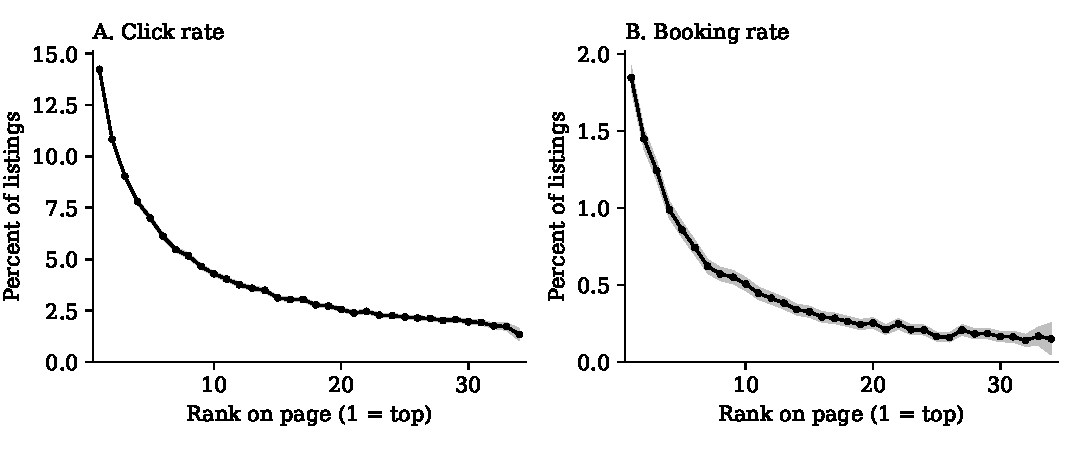
\includegraphics[width=\textwidth]{figures/position_effects.pdf}
\caption{Click and Booking Rates by Randomly Assigned Rank}
\label{fig:position}
\begin{minipage}{0.95\textwidth}\footnotesize
\textit{Notes:} Randomly ordered searches that list at least 25 hotels (73,682 searches), so that every rank is computed from the same searches. Each point is the share of listings at that rank that were clicked (panel A) or booked (panel B). Shaded bands are 95 percent confidence intervals.
\end{minipage}
\end{figure}

Table \ref{tab:position} summarizes the same pattern with estimates of equation (\ref{eq:position}), using all random searches. Ten positions lower reduces the click rate by 2.19 percentage points, 47 percent of the mean, and the booking rate by 0.32 percentage points, 59 percent of the mean. Controlling for hotel characteristics reduces these estimates by about 5 percent, to 2.09 and 0.30 percentage points, so the small imbalance in Table \ref{tab:randcheck} does not drive the results. A linear slope averages over a decline that is steep at the top and flat lower down, so it understates the loss near the top of the page and overstates it further down; the log-rank specifications, which allow for this curvature, tell the same story.

\begin{table}[htbp]
\centering
\begin{threeparttable}
\caption{Effect of Position on Clicks and Bookings}
\label{tab:position}
\small\setlength{\tabcolsep}{4pt}
\begin{tabular}{lccccc}
\toprule
 & \multicolumn{2}{c}{Click} & \multicolumn{2}{c}{Booking} & Booking, \\
\cmidrule(lr){2-3}\cmidrule(lr){4-5}
 & (1) & (2) & (3) & (4) & if clicked (5) \\
\midrule
Rank, per 10 positions & $-2.19$ & $-2.09$ & $-0.319$ & $-0.302$ & $-0.04$ \\
 & (0.015) & (0.015) & (0.005) & (0.005) & (0.22) \\[0.3em]
Log rank & $-2.79$ & & $-0.404$ & & $\phantom{-}0.03$ \\
 & (0.019) & & (0.007) & & (0.19) \\[0.3em]
Hotel characteristics & No & Yes & No & Yes & No \\
Mean of outcome (percent) & 4.66 & 4.66 & 0.539 & 0.539 & 11.57 \\
10 ranks, percent of mean & $-47$ & $-45$ & $-59$ & $-56$ & $-0.3$ \\
Listings & 2,939,652 & 2,939,652 & 2,939,652 & 2,939,652 & 136,956 \\
Searches & 121,546 & 121,546 & 121,546 & 121,546 & 121,546 \\
\bottomrule
\end{tabular}
\begin{tablenotes}\footnotesize
\item \textit{Notes:} Coefficients are in percentage points. The rank and log-rank rows come from separate regressions. All specifications include search fixed effects; standard errors clustered by search are in parentheses. Hotel characteristics are star rating, review score, log price relative to the search median, chain affiliation, location score, promotion status, and indicators for missing values. Column (5) is restricted to hotels that were clicked. Because a click is itself affected by position, this column describes the booking decision of consumers who clicked rather than estimating a causal effect.
\end{tablenotes}
\end{threeparttable}
\end{table}

\subsection{Attention or preference?}

A ranking could reduce a hotel's bookings in two ways. It could reduce the chance that consumers look at the hotel, or it could make consumers who do look at it think less of it, perhaps because they infer that a hotel shown lower must be worse. Random ordering gives that inference no basis, but consumers did not know the order was random and could still have treated a high position as a recommendation from Expedia.

Column (5) of Table \ref{tab:position} offers evidence on the two. Among hotels that were clicked, the booking rate is 11.6 percent and does not change with position: the estimate is $-0.04$ percentage points per ten positions, with a confidence interval that rules out effects larger than about 0.5 percentage points, or 4 percent of the mean. Consumers who click on a hotel low on the page book it about as often as consumers who click on a hotel at the top. The pattern is consistent with most of the booking effect operating through attention, which is also the conclusion \citet{ursu2018power} reaches with a structural model of sequential search.

This comparison should be read with care. Whether a hotel is clicked depends on its position, so the clicked hotels at the top and bottom of the page need not be comparable. Consumers who scroll far enough to click a low-ranked hotel may be unusually determined to book, which would hide a negative effect of position on how they evaluate the hotel. Column (5) describes the booking decisions of consumers who clicked; it does not by itself establish that position has no effect on evaluation.

\subsection{Which hotels depend most on placement?}

Table \ref{tab:hetero} estimates the position effect separately for four pairs of groups. Because baseline rates differ across groups, I report each slope both in percentage points and as a percent of the group's mean.

\begin{table}[htbp]
\centering
\begin{threeparttable}
\caption{Position Effects by Hotel Type}
\label{tab:hetero}
\begin{tabular}{lcccc}
\toprule
 & \multicolumn{2}{c}{Click} & \multicolumn{2}{c}{Booking} \\
\cmidrule(lr){2-3}\cmidrule(lr){4-5}
 & Per 10 ranks & Percent & Per 10 ranks & Percent \\
 & (pp) & of mean & (pp) & of mean \\
\midrule
Priced below search median & $-2.65$ (0.023) & $-51$ & $-0.392$ (0.008) & $-62$ \\
Priced above search median & $-1.74$ (0.020) & $-42$ & $-0.248$ (0.007) & $-55$ \\
\quad Difference & $-0.91$ (0.031) & & $-0.145$ (0.011) & \\[0.4em]
Chain & $-2.22$ (0.019) & $-47$ & $-0.364$ (0.007) & $-59$ \\
Independent & $-2.15$ (0.024) & $-46$ & $-0.246$ (0.008) & $-58$ \\
\quad Difference & $-0.07$ (0.031) & & $-0.118$ (0.010) & \\[0.4em]
4 or 5 stars & $-2.34$ (0.027) & $-42$ & $-0.319$ (0.009) & $-55$ \\
1 to 3 stars & $-2.00$ (0.019) & $-48$ & $-0.302$ (0.007) & $-58$ \\
\quad Difference & $-0.34$ (0.033) & & $-0.017$ (0.011) & \\[0.4em]
Review score 4.5 or higher & $-2.16$ (0.026) & $-45$ & $-0.342$ (0.009) & $-61$ \\
Review score below 4.5 & $-2.23$ (0.019) & $-48$ & $-0.321$ (0.007) & $-57$ \\
\quad Difference & $\phantom{-}0.07$ (0.033) & & $-0.021$ (0.012) & \\
\bottomrule
\end{tabular}
\begin{tablenotes}\footnotesize
\item \textit{Notes:} Each pair of rows comes from a regression of the outcome on rank, rank interacted with a group indicator, and the indicator, with search fixed effects. Slopes are in percentage points per ten positions; standard errors clustered by search are in parentheses. ``Percent of mean'' divides the slope by the group's mean outcome. The star rating comparison excludes hotels with an unknown rating; the review comparison excludes hotels with missing or zero review scores.
\end{tablenotes}
\end{threeparttable}
\end{table}

The strongest heterogeneity is by relative price. A ten-position decline reduces clicks by 51 percent of the mean for hotels priced below the search median, compared with 42 percent for hotels priced above it. The corresponding booking effects are 62 and 55 percent. Because price is unrelated to rank in the random searches (Table \ref{tab:randcheck}), this difference does not reflect where cheaper hotels happened to be placed.

By contrast, relative position effects are similar for chains and independent hotels: 47 and 46 percent for clicks, and 59 and 58 percent for bookings. In percentage points, chains lose more bookings per ten positions than independent hotels (0.36 versus 0.25), but chains are also booked more often, and the gap disappears once this is taken into account. Star ratings and review scores show the same pattern. The differences in percentage points are statistically significant with nearly three million listings, but the relative effects differ by at most about seven percentage points. There is therefore little evidence that chain affiliation, star rating, or review score substantially changes how exposed a hotel is to its position.

These data cannot say why cheaper hotels are more sensitive to position. One possibility is that consumers who scroll further down the page care less about price. Another is that consumers compare prices mainly among the hotels they see first, so that a low price helps a hotel most when it is near the top. Distinguishing these explanations would require information on which listings consumers actually viewed, not only which ones they clicked.

% =============================================================================
\section{Conclusion}
% =============================================================================

Expedia's random ordering experiment shows that a hotel's position on a results page has a large effect on whether consumers consider it. Among searches displaying at least 25 hotels, moving from first to fifth position reduces click and booking rates by about half, and moving from first to tenth reduces them by about two-thirds. Most of this loss occurs in the first few positions.

The results point to attention as the main channel. Among hotels that consumers click, booking rates vary little with position, although this comparison is not itself causal. Position effects also vary with relative price: hotels priced below others in the same search are more sensitive to where they appear, while relative effects are similar for chain and independent hotels and across measures of hotel quality.

The results show how much a platform can shift consumer attention simply by changing the order in which it presents alternatives. For a hotel, the difference between appearing first and appearing fifth is roughly half of the consumers who would otherwise click on it or book it.

% =============================================================================
\bibliographystyle{apalike}
\bibliography{references}

\clearpage
\appendix
\setcounter{table}{0}
\renewcommand{\thetable}{A\arabic{table}}
\section*{Appendix}

\begin{table}[htbp]
\centering
\begin{threeparttable}
\caption{Search Characteristics by Ranking Arm in the Released Data}
\label{tab:sampling}
\begin{tabular}{lccc}
\toprule
 & Algorithmic & Random & Standardized \\
 & order & order & difference \\
\midrule
\multicolumn{4}{l}{\textit{Chosen before results are shown}} \\
\quad Length of stay (nights) & 2.16 & 2.94 & $-0.35$ \\
\quad Booking window (days) & 32.99 & 49.57 & $-0.30$ \\
\quad Adults & 1.95 & 2.05 & $-0.12$ \\
\quad Children & 0.37 & 0.39 & $-0.03$ \\
\quad Rooms & 1.13 & 1.12 & $\phantom{-}0.02$ \\
\quad Includes a Saturday night & 0.51 & 0.48 & $\phantom{-}0.06$ \\
\quad Has purchase history & 0.063 & 0.029 & $\phantom{-}0.16$ \\
\quad Domestic search & 0.65 & 0.60 & $\phantom{-}0.10$ \\[0.3em]
\multicolumn{4}{l}{\textit{Outcomes}} \\
\quad Clicks per search & 1.10 & 1.13 & $-0.04$ \\
\quad Search ends in a booking & 0.939 & 0.130 & \\[0.3em]
Searches & 277,798 & 121,546 & \\
\bottomrule
\end{tabular}
\begin{tablenotes}\footnotesize
\item \textit{Notes:} One observation per search; all searches in the released training data. The standardized difference is the difference in means divided by the pooled standard deviation. Every released search contains at least one click.
\end{tablenotes}
\end{threeparttable}
\end{table}

\end{document}
